\documentclass[11pt, a4paper]{article}		% general format


%%%% Charset
\usepackage[utf8]{inputenc}					% use utf8					
\usepackage[russian]{babel}					% use russian font


%%%% Math
\usepackage{amsmath}						% Amer­i­can Math­e­mat­i­cal So­ci­ety (AMS) math fa­cil­i­ties
\usepackage{amsfonts}						% fonts from the AMS
\usepackage{amssymb}						% additional math symbols


%%%% Graphics
\usepackage{graphicx}


\author{Дедков Сергей}
\title{Отчет по лабораторной работе №1 :\\ \LaTeX{}, Git, GPG}
\date{2015}

%---------------------------------------------------------

\begin{document}
\maketitle
\tableofcontents
\newpage

%---------------------------------------------------------


\section{Цель работы}

Определить набор и версии сервисов запущенных на компьютере в диапазоне адресов.
Данная работа выполняется на ОС kali linux, используется утилита nmap.



%---------------------------------------------------------

\section{Ход работы}


%---------------------------------------------------------

\subsection{Провести поиск активных хостов}

Так как наш компьюер находиться в подсети 192.168.76.0/24 выполним поиск в ней(для определения воспользовались командой ifconfig). Для этого воспользуемся командой nmap 192.168.76.0/24.
В результате видим 5 хостов, один из них - виртуальная машина с запущенной metasploit, а именно с ip адресом 192.168.76.136. См. рисунок 1.

\begin{figure}[h!]
\centering
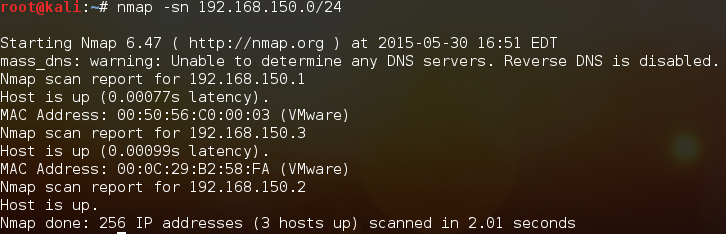
\includegraphics[scale=0.75]{res/hosts_search}
\caption{Поиск хостов}
\end{figure}

%---------------------------------------------------------

\subsection{Определить открытые порты}

Для определения открытых портов достаточно просто ввести nmap 192.168.76.136 (сканируются порты до 1024). Или же воспользоваться опцией -p, например nmap -p "*" 192.168.76.136. Данной командой просканируются все порты, если необходимо задать диапазон достаточно указать его вместо "*".
После ввода команды увидим результат, как на рисунке 2.

\begin{figure}[h!]
\centering
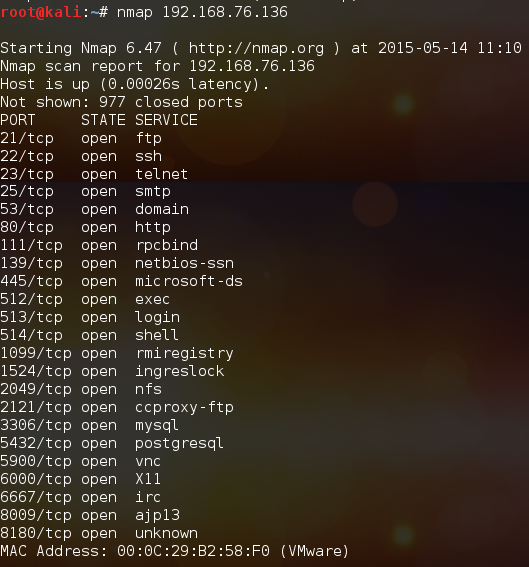
\includegraphics[scale=0.75]{res/ports_scan}
\caption{Поиск портов}
\end{figure}

%---------------------------------------------------------

\subsection{Определить версии сервисов}

Чтобы определить версии сервисов необходимо воспользоваться командой nmap с ключем sV следующим образом: nmap -sV 192.168.76.136. На рисунке 3 можно увидеть результат.

\begin{figure}[h!]
\centering
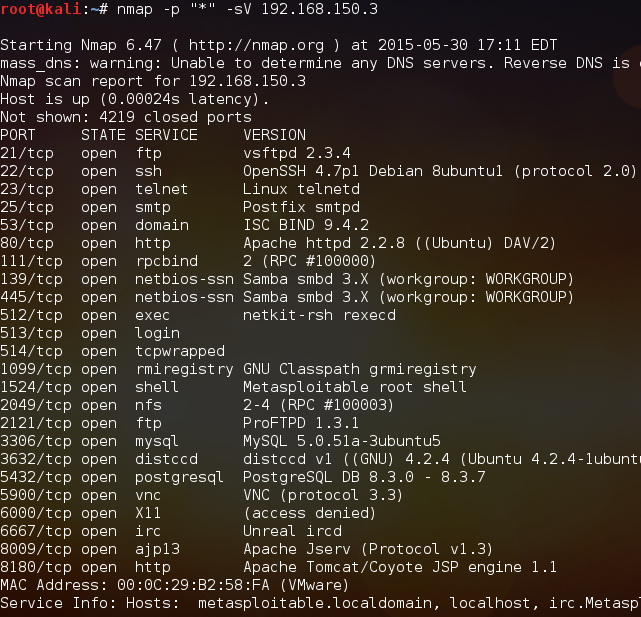
\includegraphics[scale=0.75]{res/services_versions}
\caption{Определение версий сервисов}
\end{figure}

%---------------------------------------------------------

\subsection{Изучить файлы nmap-services, nmap-os-db, nmapservice-probes}

Рассмотрим файл nmap-services. Для этого введем команду 

vim /usr/share/nmap/nmap-services. 

Файл служит для быстрого поиска, напрмер с ключем -F. В файле в каждой строчке задаются сервисное название или сокращение, число порта и протокол, определенный разделом, частота порта мера того, как часто порт был найдет открытым во время сканирования. Пример файла можно увидеть на рисунке 4.


\begin{figure}[h!]
\centering
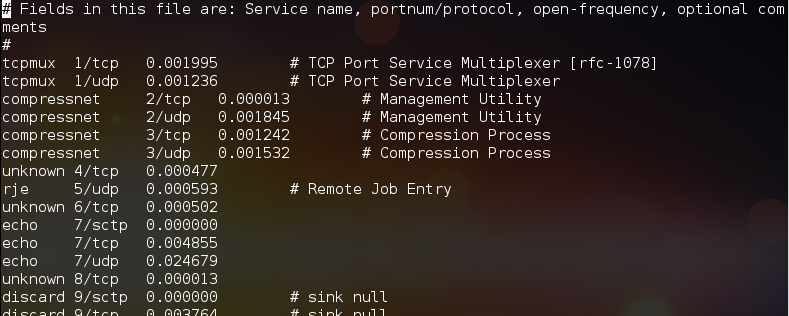
\includegraphics[scale=0.75]{res/nmap_services}
\caption{Файл nmap-services}
\end{figure}

Файл nmap-os-db содержит сотни примеров реакций ОС на nmap. Таким образом nmap определяет какая опреационная система установлена на удаленной машине. Для того чтобы узнать какая ОС установлена нужно запустить nmap с ключем -O. Содержимое файла представлено на рисунке 5.

\begin{figure}[h!]
\centering
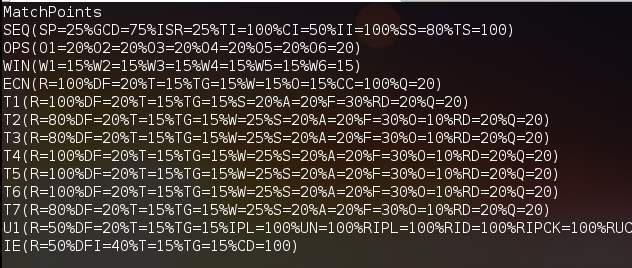
\includegraphics[scale=0.75]{res/nmap_os_db}
\caption{Файл nmap-os-db}
\end{figure}


nmap-service-probes — это простой текстовый файл состоящий из строк, в котором хнаняться тесты и сигнатуры подсистем определений версий. Строки, начинающиеся с символа "решетки" (\#) воспринимаются как комментарии и игнорируются обработчиком. Пустые строки также не обрабатываются. 


Синтаксис: 
\begin{itemize}
\item Probe <protocol> <probename> <probesendstring> - директива probe (тест) - указывает nmap, какие данные отправлять в процессе определения служб
\item match <service> <pattern> <productname> <version> <device> <h?????> <info> <OS> - указывает nmap на то, как точно определить службу, используя полученный ответ на запрос, отправленный предыдущей директивой probe. Эта директива используется в случае, когда полученный ответ полностью совпадает с шаблоном. При этом тестирование порта считается законченным, а при помощи дополнительных спецификаторов nmap строит отчет о названии приложения, номере версии и дополнительной информации, полученной в ходе проверки
\item softmatch <service> <pattern> <productname> <version> <device> <h?????> <info> <OS> - имеет аналогичный формат директиве match. Основное отличие заключается в том, что после совпадения принятого ответа с одним из шаблонов softmatch, тестирование будет продолжено с использованием только тех тестов, которые относятся к определенной шаблоном службе. Тестирование порта будет идти до тех пор, пока не будет найдено строгое соответствие (match) или не закончатся все тесты для данной службы
\item ports <portlist> - группирует порты, которые обычно закрепляются за идентифицируемой данным тестом службой
\item sslports <sslportlist> - аналогична директиве ports, только эта директива указывает порты, обычно используемые совместно с SSL
\item totalwaitms <milliseconds> - редко используемая, т.к. указывает сколько времени (в миллисекундах) необходимо ждать ответ, прежде чем прекратить тест службы
\end{itemize}

%---------------------------------------------------------

\subsection{Добавить новую сигнатуру службы в файл nmap-service-probes (для этого создать минимальный tcp server, добиться, чтобы при сканировании nmap указывал для него название и версию)}

Напишем простой tcp-сервер, который просто ждет подключения клиента и отправляет ему сообщение. В файл nmap-service-probes добавим следующую строку: 

\verb"match tcp-server m|^111| v/1.0.X/ p/Dedkov S.V./ i/It's works /"

Код сервера:

\begin{verbatim}
using System;
using System.Collections.Generic;
using System.Linq;
using System.Text;
using System.IO;
using System.Net;
using System.Net.Sockets;
using System.Threading;

namespace ExampleTcpListener_Console
{
    class ExampleTcpListener
    {
        static void Main(string[] args)
        {
            TcpListener server = null;
            try
            {
                int MaxThreadsCount = Environment.ProcessorCount * 4;
                Console.WriteLine(MaxThreadsCount.ToString());
                ThreadPool.SetMaxThreads(MaxThreadsCount, MaxThreadsCount);
                ThreadPool.SetMinThreads(2, 2);

                Int32 port = 9596;
                IPAddress localAddr = IPAddress.Parse("192.168.137.1");
                int counter = 0;
                server = new TcpListener(localAddr, port);

                server.Start();

                while (true)
                {

                    Console.Write("\nWaiting for a connection... ");

                    ThreadPool.QueueUserWorkItem(ObrabotkaZaprosa, server.AcceptTcpClient());
                    counter++;
                    Console.Write("\nConnection №" + counter.ToString() + "!");

                }
            }
            catch (SocketException e)
            {
                Console.WriteLine("SocketException: {0}", e);
            }
            finally
            {
                server.Stop();
            }
            
            Console.WriteLine("\nHit enter to continue...");
            Console.Read();
        }

        static void ObrabotkaZaprosa(object client_obj)
        {
            Byte[] bytes = new Byte[256];
            String data = null;

            TcpClient client = client_obj as TcpClient;

            data = null;

            NetworkStream stream = client.GetStream();

            int i;

            data = "111";
            byte[] msg = System.Text.Encoding.ASCII.GetBytes(data);
            stream.Write(msg, 0, msg.Length);

            client.Close();
        }
    }
}
\end{verbatim}
  
Таким образом теперь nmap знает, что если при пустом запросе с сервера прихоит строка 111, значит нужно выводить информацию которая указана на рисунке 6.

\begin{figure}[h!]
\centering
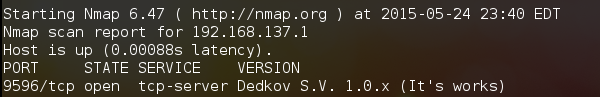
\includegraphics[scale=0.75]{res/server_response}
\caption{Вывод информации о сервисе}
\end{figure}



%---------------------------------------------------------

\subsection{Сохранить выводы утилиты в формате xml}

Для того, чтобы вывести данные в xml файл достаточно вызвать команду nmap с ключем -oX и указать имя файла. Например: 

\verb'namp -sn -oX output.xml 192.168.137.1'

Результат можно увидеть на рисунке 7:

\begin{figure}[h!]
\centering
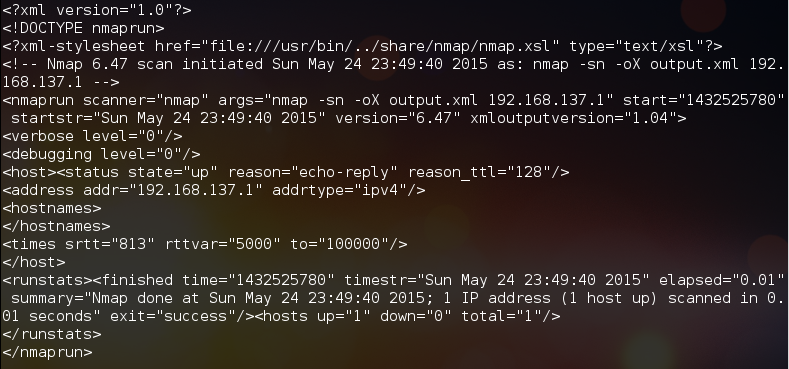
\includegraphics[scale=0.75]{res/xml_output}
\caption{output.xml}
\end{figure}

%---------------------------------------------------------

\subsection{Исследовать различные этапы и режимы работы nmap с использованием утилиты Wireshark}

Запустим утилиту Wireshark, выберем интерфейс eth0 и нажмем Start. Будет произведено сканирование сети и вывод передаваемых по сети пакетов. Пропингуем с ОС Metasploitable2 основную ОС и проверим, будет ли утилита Wireshark видеть подобную активность сети? Как видно из рисунка 14, утилита отображает информацию об активности в сети. Так же можно посмотреть информацию о соединении и передаваемых пакетах, а в некоторых случаях и перехватить cookie.

%---------------------------------------------------------

\subsection{Просканировать виртуальную машину Metasploitable2 используя nmap\_db из состава metasploit-framework}

Запустив metasploit, мы можем воспользоваться командой nmap\_db


%---------------------------------------------------------

\subsection{Выбрать пять записей из файла nmap-service-probes и описать их работу. Выбрать один скрипт из состава Nmap и описать его работу}

\begin{itemize}
\item Первая запись

Возьмем самую первую запсись prode - эта запись теста с отправкой null-запроса. В данной записи будет отправляться пустой запрос по протоколу TCP. С ожиданием ответа в 6 секунд(директива totalwaitms).

\begin{figure}[h!]
\centering
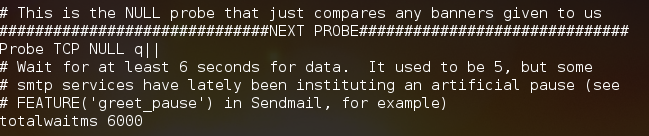
\includegraphics[scale=0.75]{res/probe_1}
\caption{Запись 1}
\end{figure}

\item Вторая запись

Второй записью рассмотрим match после probe null-запроса. Если пользователь укажет ключ -sV при использовании nmap и после отправки нулевого теста с сервера приедет выражение подходящее под mSxf5xc6x1a тогда в колонке SERVICE при выводе информации он увидит наименование сервиса 1c-server, а в олонке VERSION 1C:Enterprise business management server.

\begin{figure}[h!]
\centering

\includegraphics[scale=0.75]{res/probe_2}
\caption{Запись 2}
\end{figure}

\item Третья запись

В данной запись на сервер отправляется запрос по протоколу TCP в котором передается информация. Так же 



\begin{figure}[h!]
\centering
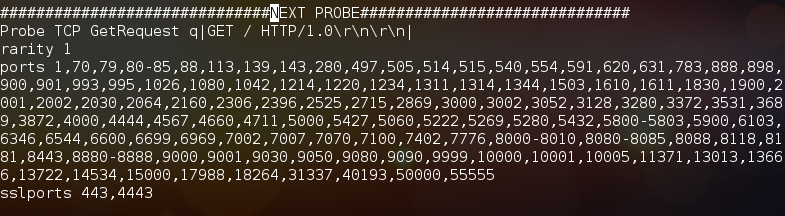
\includegraphics[scale=0.75]{res/probe_3}
\caption{Запись 3}
\end{figure}



\end{itemize}









\end{document}